\chapter{Introducción}

\section{¿Qué es la materia condensada?}

\begin{itemize}
    \item Fases condensadas: aparecen cuando los sistemas f\'isicos est\'an formados por un n\'umero grande de elementos que interact\'uan fuertemente.
    \item Fases condensadas bastante conocidas: s\'olidos, l\'iquidos.
    \item Otras fases condensadas: superconductores, superfluidos, ferromagnetos, antiferromagnetos, condensados Bose-Einstein.
    \item Otras mesofases: cristales líquidos, membranas autoensambladas, geles, coloides, cristales, vidrios, etc.
\end{itemize}

Categorías de la física:
\begin{itemize}
    \item Teórico
    \item Experimental
    \item Fenomenológica
    \item Computacional
\end{itemize}

\subsection{De la física del estado sólido a la física de la materia condensada}

\begin{itemize}
    \item La física del estado sólido en los 30 (siglo XX):
    \begin{itemize}
        \item Cristalografía por Rayos X
        \item Difracción de electrones
        \item M cuántica + M estadística
    \end{itemize}
\end{itemize}

\subsection{Tipos de fuerzas}


\begin{itemize}
    \item Van der Waals
    \item Interacción electromagnética
    \item Interacción de intercambio
    \item Potencial de London
    \item Potencial de Lenard-Jones
\end{itemize}

\section{¿Qué estudia la materia condensada?}

Se vale de muchos métodos para estudiar la materia. 
\begin{itemize}
    \item Mecánica estadística
    \begin{itemize}
        \item Modelo de campo medio
        \item Movimiento Browniano
        \item Dinámica molecular
    \end{itemize}
    \item Mecánica cuántica
    \begin{itemize}
        \item Modelo de Hubbard (1963-1966)
        $$\hat{H}=-t\sum_{\langle i,j\rangle\sigma}\left(C_{i\sigma}^\dagger C_{j\sigma}+C_{j\sigma}^\dagger C_{i\sigma}\right)+U\sum_{i}n_{i\uparrow}n_{i\downarrow}$$
        Donde:
        \begin{itemize}
            \item $C_{i\sigma}^\dagger$: Operador bosónico de creación de partículas de espín $\sigma$ en la posición $i$.
            \item $C_{j\sigma}$: Operador bosónico de aniquilación de partículas de espín $\sigma$ en la posición $j$.
            \item $n_i$: Operador número en la posición $i$.
        \end{itemize}
    \end{itemize}
\end{itemize}

\textbf{Un mol} es $6.022E23$.

\subsection{Objetivo de la materia condensada}
\begin{itemize}
    \item El objetivo de la Física de la materia condensada es el entendimiento de las propiedades de grandes conjuntos de átomos y moléculas en términos de las interacciones entre ellas.
    \item Propiedades macroscópicas
    \begin{itemize}
        \item Temperatura
        \item Presión
        \item Volumen
        \item Energía de enlace
        \item Opacidad
    \end{itemize}
    \item De lo más notable de la física de la materia condensada, es el poder explicar la fenomenología de un sistema que surge de un Hamiltoniano relativamente simple.
\end{itemize}

\subsection{Hitos de la física de la materia condensada}

\begin{itemize}
    \item Efecto fotoeléctrico (Einstein, 1905)
    \item Capacidad Calorífica (Einstein, 1907)
    \item Ferromagnetismo (Weiss, 1907)
    \item Licuefacción de He @ 4.1K (Kemerling Onnes, 1908)
    \item Superconductividad (Kamerling Onnes, 1911) 
    \item Difracción de Rayos X (Von Laue, 1912)
    \item Cuantización de las vibraciones de una red cristalina (Max Born, 1912)
    \item Corrección de la aproximación de la capacidad calorífica (Debye, 1912)
    \item Ecuación de Schrodinger (Schrodinger, 1926)
    \item Principio de exclusión de Pauli (Pauli, 1926)
    \item Aproximación Born-Oppenheimer (1927) Desacoplan dinámicas de núcleos y electrones.
    \item Descripción cuántica del modelo de electrones libres (Sommerfeld, 1928)
\end{itemize}

\subsection{Materia Blanda y Materia Sólida}

Orden (desorden) estadístico:

\begin{align*}
    \text{Entropía}\\
    S=-k\log\omega
\end{align*}

\begin{figure}[H]
    \centering
    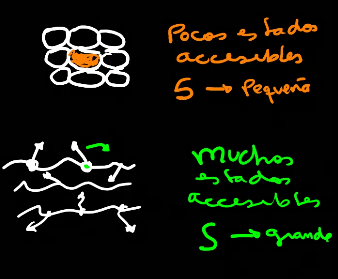
\includegraphics[width=0.4\textwidth]{Graficas/Jul27-1.png}
    \caption{Sólidos ordenados, líquidos desordenados}
    \label{fig:SolLiq}
\end{figure}

Tres categorías:

\begin{enumerate}
    \item Orden de largo alcance
    \item Orden de corto alcance
    \item Desorden
\end{enumerate}


\textbf{Materia blanda:}

\begin{itemize}
    \item Escalas de longitud: Desde escalas atómicas a escalas macroscópicas.
    \item Fluctuaciones
    \item Autoreorganización


\item\textbf{Macroscópicas}

\begin{itemize}
    \item Polímeros
    \item Interfaces
\end{itemize}

\item\textbf{Microscópicas}

\begin{itemize}
    \item Coloides
    \item Geles 
    \item Cristales líquidos
\end{itemize}

\end{itemize}

\subsubsection*{Fluctuaciones y Movimiento Browniano}

\begin{itemize}
    \item Partes pequeñas que tienen movimiento aleatorio
    \item Fluctuaciones térmicas
\end{itemize}

\subsection{Materia sólida} 

Cristalografía clásica: Sistemas que se representan como puntos con patrons específicos.
\begin{itemize}
    \item Grupos de traslación (redes Bravais)
    \item Traslación y simetría (grupos de Schontlis)
\end{itemize}


\subsection{Fases de la materia}

\begin{tabular*}{0.8\textwidth}{l|rl}
             & Ordenadas & No ordenadas\\
             \hline
     Clásica & Hielo de agua & Agua líquida\\
     Cuántica & Ferromagnética\\
                & Antiferromagnética\\
\end{tabular*}

\subsection{Conjuntos de puntos:}

\begin{itemize}
    \item Conjunto unitario: tiene un solo elementos.
    \item La union contable de conjuntos unitarios suma un conjunto de puntos.
    \item Un conjunto de puntos, $\Lambda\subset \mathbb{R}^d$, es un conjunto discreto si $x\in \Lambda$ tiene una vecindad abierta $U=U(x)\subset \mathbb{R}^d$ que no tiene ningún elemento de $\Lambda$.
    \item Para cada $x\in\Lambda$, exite un radio de empaquetamiento $r>0$ tal que $B(r)$ es una hiperesfera de radio $r$ tal que $B_r(x) \cap \Lambda=\{x\}$.
    \item Por otro lado, $\Lambda$ es uniformemente discreto si hay una vecindad abierta, $U$, de $0\in\mathbb{R}^d$ tal que $(x+U)\cap(y+U)=\emptyset$. Se cumple para todo $x,y\in\Lambda$ la suma y diferencia de Minkowski para dos conjuntos $U\pm V:=\left\{u\pm v \lvert u \in U,v\in V\right\}$
    \item Para un conjunto discreto se tiene una distancia mínima entre puntos. Los subconjuntos de $\mathbb{Z}$ son uniformemente discretos. Pero podemos construir conjuntos discretos no uniformes, por ejemplo: $A=\left\{\frac{1}{n}\lvert n\in \mathbb{N}\right\}$
    \item Un conjunto $\Lambda$ es localmente finito, si para todos los conjuntos $K\subset \mathbb{R}^d$, $K\cap\Lambda$ es un conjunto finito o $\emptyset$. 
    ``Cuando $\Lambda$ es un conjunto de puntos, también es localmente finito si y solo si es discreto y cerrado.'' Además, $\Lambda$ es relativamente denso si existe un conjunto compacto $K\subset \mathbb{R}^d$ tal que $\Lambda+K=\mathbb{R}^d$.
    \item Un conjunto de puntos $\Lambda\subset\mathbb{R}^d$ es un conjunto de Delone (Delany), ``un Delone'' si es uniformemente discreto y relativamente denso.
    \item Para cualquier conjunto de Delone, $\Lambda\subset \mathbb{R}^d$ se puede elegir un radio de empaquetamiento $r$ y otro de ``recubrimiento'', $R$ tal que $U=B_r(0)$ (hiperesfera) y $K=\overline{B_R(0)}$ son vecindades apropiadas para confinar $\Lambda$.
    \item Un conjunto de puntos $\Lambda\subset \mathbb{R}^d$ es un conjunto de Meyer, ``un Meyer'', si $\Lambda$ es relativamente denso y $\Lambda-\Lambda$ es uniformemente discreto.
    \item Todos los conjuntos de Meyer son de Delone, pero no todos los conjuntos de Delone son de Meyer.
\end{itemize}

\textbf{Por ejemplo:}

\begin{align*}
    \Lambda&=\left\{n+\frac{1}{n}\rvert n \in \mathbb{Z}\backslash 0\right\}\\
        &=\left\{2,2\frac{1}{2},3\frac{1}{3},\cdots\right\}
\end{align*}

\begin{itemize}
    \item Es uniformemente discreto.
    \item Tiene un radio de empaquetamiento $r=1/4$
    \item Es relativamente denso
    \item Radio de recubrimiento $R=2$
\end{itemize}

Es un conjunto de Delone.
No es un conjunto de Meyer.

\begin{itemize}
    \item Un conjunto de puntos $\Gamma \subset \mathbb{R}^d$ son puntos de red (grid). O simplemente una red en $\mathbb{R}^d$ si existen $d$ vectores $\vec{b}_1,\cdots,\vec{b}_d$ tal que
    $$
        \Gamma=\mathbb{Z}b_1\oplus\cdots\oplus\mathbb{Z}b_d:=\left\{\sum_{i=1}^dm_ib_i\lvert\forall m_i\in\mathbb{Z}\right\}
    $$
    y que además, si $\mathbb{R}^d$ es generado por $\left\{b_1,\cdots,b_d\right\}$ es una base de la red $\Gamma$. Es un conjunto de Meyer, y consecuentemente, es un conjunto de Delone.
\end{itemize}

\subsubsection{Celda de Voroni y celda de Delone:}

Considere un conjunto de puntos localmente finito $\Lambda\subset \mathbb{R}^d$ y $\Lambda\neq\emptyset$. Entonces el dominio de Voronoi o celda de Voronoi para $a\in\Lambda$ es $V(a):=\left\{x\in\mathbb{R}^d\vert\norm{x-a}\leq\norm{x-b}\forall b\in\Lambda\right\} $

Donde $\norm{\bullet}$ es la métrica euclideana.

$V(a)$ es cerrada en volumen y es abierta en muchas ocasiones en las fronteras.

$V(a)$ tiene un hipervolumen finito y no nulo.

$V(a)$ no necesariamente es compacta. ($A\cup B=$Universo, $A\cap B=\emptyset),\Rightarrow A$ es compacto).

La colección de todas las celdas de Voronoi forman una teselación cara a cara de $\mathbb{R}^d$.

En particular, dos celdas de Voronoi distintas pueden intersectarse.

El conjunto de celdas forma un espacio euclidano llamado Complejo de Voronoi.

El dual geométrico del complejo de Voronoi, es otro conjunto de celdas de Delone y se llama Complejo de Delone.


\subsection{Grupos finitos:}

\begin{itemize}
    \item En cristalografía son importantes los grupos de moléculas
    \item Grupo lineal general en $\mathbb{R}^d$ $GL(d,\mathbb{R})$:
    Todas las matrices de dimensión $d\times d$ y que todas sus entradas son invertibles.
    \item Grupo ortonormal especial o grupo de rotación: el subgrupo de rotaciones que preservan la orientación.
\end{itemize}

\textbf{Grupos finitos más usados en cristalografía}
\begin{itemize}
    \item Grupo cíclico de orden $n$, $C_n$ que satisface que si $g^n=e$ entonces $g^{ln}=e\forall l \in \mathbb{Z}$ y $e:$ elemento neutro.
    \item Grupo didral de orden $2n$:
    $$D_n=\bra*{g,h}\ket*{g^n=h^2=(gh)^2=e}$$
    \item 4-grupo de Kein.
    $$D_2=C_2\times C_2$$
    \item Grupo de permutación: tiene $n$ símbolos $S_n$, para $n>1$ su subgrupo de índice $2$ permutaciones se llama grupo alternado o alternante.
    $$A_n=\left\{\sigma\in S_n:\norm{\sigma}\text{ es par}\right\}$$
    \item Grupos de simetría de politopos regulares:
    
    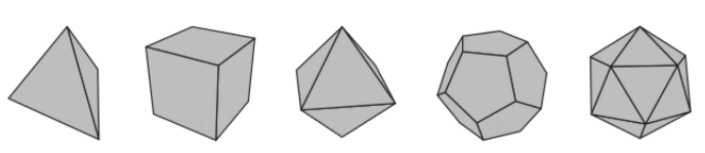
\includegraphics[width=0.4\textwidth]{Graficas/Aug6-1.png}
    \begin{itemize}
        \item Grupo tetraedro $T_d\approxeq S_4$: rotaciones y reflecciones del tetraedro.
        \item Grupo octaedro $O\approxeq S_4$: Preserva orientaciones de cubo y octaedro.
        \item Grupo icosaedro $Y_h=Y\times C_2$: $Y$ subgrupo de rotaciones.
    \end{itemize}
\end{itemize}


\subsection{Cálculo de las celdas de Voronoi y de Delone}

Propiedades de la celda de Voronoi $V(a)$:

\begin{enumerate}
    \item Es una celda cerrada.
    \item Hipervolumen no nulo.
    \item No es necesariamente compacta.
    \item Cada punto de conjunto de puntos tiene su propia celda.
\end{enumerate}

El conjunto de celdas de Voronoi forma un complejo de Voronoi, que es una teselación del espacio.

El dual geométrico del complejo de Voronoi se llama complejo de Delone.

Se llama celda de Voronoi en honor de Georgy  Voronoi (1868-1908).

Se llama celda de Delone en honor a Boris Delone (1890-1980).


\subsubsection{Algoritmo de Fortune}

Propuesto por Steve Fortune. 

\textit{Entrada:} El conjunto de puntos $\left\{p_1,\cdots,p_n\right\}$. El índice del punto donde se calcula 

\textit{Salida:} La celda de Voronoi.

\begin{enumerate}
    \item Iniciar
    \item $cell_i\leftarrow S$
    \item $P_i\leftarrow (x_i,y_i)$
    \item Para todos los puntos $i\neq j$ hacer:
    \begin{enumerate}
        \item $P_j\leftarrow (x_i,y_i)$
        \item $R_j\leftarrow $ linea que une $P_i$ y $P_j$.
        \item $PM_i\leftarrow$ punto medio entre $P_i$ y $P_j$.
        \item $\bar{R}_j\leftarrow$ línea perpendicular a $R_j$ en $PM_i$
        \item Hallar la intersección de $cell_i$ y $\bar{R}_j$.
        \item Si $R_j$ y $L$ se cruzan en $0$ o $1$ punto, continua.
        \item Si no, $cell_i\leftarrow$
    \end{enumerate}
\end{enumerate}


\chapter{Estructuras cristalinas y enlaces cristalinos}

\begin{enumerate}
    \item Red cristalina y tipos de cristales.
    \item Redes de Bravais.
    \item Planos cristalinos.
    \item Indices de Miller.
    \item Análisis cristalográfico.
    \item Factor de dispersión.
    \item Factor geométrico de estructura.
    \item Red recíproca.
    \item Enlaces en cristales de gases inertes (iónicos, metálicos, covalentes).
\end{enumerate}

\section{Red (estructura) cristalina y tipos de cristales}

\subsection{Los sólidos:}
\begin{itemize}
    \item Los sólidos presentan una estructura cristalina ordenada.
    
    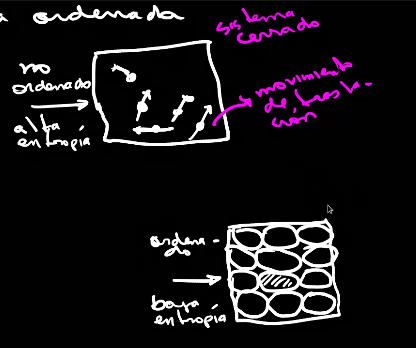
\includegraphics[width=0.4\textwidth]{Graficas/Aug17-1.png}
\end{itemize}

\section{Redes de Bravais}

La estructura cristalina se estudia mediante las redes de Bravais.

\begin{itemize}
    \item Pueden ser en $1D$, $2D$, y $3D$.
    \item La periodicidad de la red era desconocida antes del análisis con Rayos X.
    
    $\rightarrow$ la regularidad de los cristales macroscopicos debía seguir a nivel micro.
    
    La confirmación experimental viene de $1913$ cuando Bragg estudia la difracción de rayos X por estas estructuras.
    \item Las redes de Bravais especifican los arreglos periódicos en los cuales se repiten las unidades cristalinas.
    \item Estas unidades cristalinas pueden ser átomos (cristal atómico), moléculas (cristal molecular), grupos de átomos, grupos de moléculas, iones, grupos de iones, etc.
    \item La red de Bravais resume la geometría del cristal, y es independiente de las unidades cristalinas.
\end{itemize}

\textit{``Una red de Bravais es un conjunto infinito de puntos discretos con un arreglo y orientación que parece exactamente la misma desde cualquier punto.''}

\textit{``Una red tridimensional de Bravais es el conjunto de puntos dados por el vector de posición $\vec{R}=n_1\hat{a}_1+n_2\hat{a}_2+n_3\hat{a}_3$ donde $n_1,n_2,n_3~\in\mathbb{Z}$ y  $\hat{a}_1,\hat{a}_2,\hat{a}_3$ son vectores no-coplanares, se llaman vectores primitivos y son una base de $\mathbb{R}^3$.''}

\begin{itemize}
    \item Una base de un espacio genera un conjunto de puntos que pertenecen al espacio. Los elementos de la base son LI. Todo elemento del espacio se puede escribir como una combinación lineal de los elementos de la base.
    \item Aunque el térmico ``Red de Bravais'' corresponde al conjunto de puntos, también se usa para refriese al conjunto de vectores que unen estos puntos, y también al conjunto de las traslaciones determinadas por esos vectores. 
    \item La red de Bravais en $1D$ es: $\gamma:=\left\{m_1\vec{b}_1\lvert\forall m_1, \in \mathbb{Z}\right\}$
\end{itemize}

\subsection{Número de coordinación}

\begin{itemize}
    \item En una red de Bravais, los puntos más cercanos a un punto de interés son sus próximos vecinos y dada la periodicidad de la red, cada punto tiene el mismo número de próximos vecinos y este es un número de coordinación.
\end{itemize}

\subsection{Celda primitiva}

\begin{itemize}
    \item El paralelepípedo definido por los ejes del cristal (vectores primitivos) se llama celda primitiva.
    \item Usando el conjunto de traslaciones, la celda primitiva llena el espacio. La celda primitiva forma una teselación del espacio.
    \item Hay muchas formas de elegir vectores primitivos. pero vamos a llamar celda primitiva a la celda de menor hipervolumen.
    \item Siempre hay un punto de la red por celda primitiva.
    \item El hipervolumen de la celda es:
    $$V_c=\abs*{\vec{a}_1\cdot\hat{a}_2\times\hat{a}_3}$$
\end{itemize}

\textbf{Simetrías:}

\begin{itemize}
    \item[nel] Continuas: Grupos de Lie.
    \item[si] Discretas: Grupos finitos.
\end{itemize}

% \section{Planos Cristalinos}

% \section{Indices de Miller}

% \section{Análisis cristalográfico}

% \section{Factor de dispersión}

% \section{Factor geométrico de estructura}

% \section{Red recíproca}

% \section{Enlaces en cristales de gases inertes (iónicos, metálicos, covalentes)}

